%
% Portuguese-BR vertion
% 
\documentclass{article}

\usepackage{ipprocess}
% Use longtable if you want big tables to split over multiple pages.
% \usepackage{longtable}
\usepackage[utf8x]{inputenc} 
\usepackage[brazil]{babel} % Uncomment for portuguese
\usepackage{graphicx}

\sloppy

\graphicspath{{./pictures/}} % Pictures dir
\makeindex
\begin{document}

\DocumentTitle{Documento de Requisitos}
\Autor {Gleidson Vinícius Gomes Barbosa - 6331}
\Project{Sistema para Locadora de jogos}
\Organization{Universidade Federal de Viçosa - Campus Rio Paranaíba}

\capa
%\newpage

%%%%%%%%%%%%%%%%%%%%%%%%%%%%%%%%%%%%%%%%%%%%%%%%%%
%% Revision History
%%%%%%%%%%%%%%%%%%%%%%%%%%%%%%%%%%%%%%%%%%%%%%%%%%
%\section*{\center Histórico de Revisões}
  %\vspace*{1cm}
  %\begin{table}[ht]
   % \centering
    %\begin{tabular}[pos]{|m{2cm} | m{7.2cm} | m{3.8cm}|} 
     % \hline
      %\cellcolor[gray]{0.9}
      %\textbf{Date} & \cellcolor[gray]{0.9}\textbf{Descrição} & %\cellcolor[gray]{0.9}\textbf{Autor(s)}\\ \hline
      %%\hline
      %\small 27/10/2019 & \small Criação do documento. & \small %Gleidson Vinícius Gomes Barbosa \\ \hline \small 12/11/2019 &
      %\begin{small}
      %  \begin{itemize}
       %   \item Gleidson Vinícius Gomes Barbosa;
        %  \item Matrícula - 6331.
        %\end{itemize}
      %\end{small} & \small Gleidson Vinícius Gomes Barbosa \\ \hline 
    %\end{tabular}
  %\end{table}

%\newpage

% TOC instantiation
\tableofcontents
\newpage

%%%%%%%%%%%%%%%%%%%%%%%%%%%%%%%%%%%%%%%%%%%%%%%%%%
%% Document main content
%%%%%%%%%%%%%%%%%%%%%%%%%%%%%%%%%%%%%%%%%%%%%%%%%%
\section{Introdução}
\subsection{Propósito}
O sistema irá gerenciar uma Locadora de jogos que também permite o uso de consoles de jogos no local, assim auxiliando no controle de estoque, clientes, funcionários e máquinas do local.

\subsection{Escopo}
    O sistema deve gerenciar o estoque, observando a disponibilidade de produtos, reservas e detalhes de cada produto; os clientes, observando todos os seus dados, restrições, pendências e casos especiais; e os funcionários, observando seus dados, restrições, horário de trabalho, atividades durante o horário de trabalho.
    
  % inicio da tabela de acronimos e abreviacoes do documento
  \subsection{Acrônimos e Abreviações}
    \FloatBarrier
    \begin{table}[H]
      \begin{center}
        \begin{tabular}[pos]{|m{2cm} | m{12cm}|} 
          \hline
          \cellcolor[gray]{0.9}\textbf{Sigla} & \cellcolor[gray]{0.9}\textbf{Descrição} \\ \hline
          FR      & Requisito Funcional  \\ \hline
          NFR     & Requisito Não Funcional  \\ \hline
          CE      & Casos Especiais  \\ \hline
        \end{tabular}
      \end{center}
    \end{table}  
  % fim
    
\subsection{Visão Geral do Documento}
  \begin{itemize}
   \item \textbf{Descrição Geral} - Descreve o produto e suas funções.
   \item \textbf{Requisitos Específicos} - Descreve detalhadamente os requisitos do sistema.
  \end{itemize}


  \section{Descrição Geral}
    \subsection{Perspectiva do Produto} 
    %Descrever os relacionamentos do produto com: sistema, usuário, hardware, software, comunicação, etc.
    O Sistema deverá ter dois tipos de interface, sendo uma para o cliente e uma para o funcionário e deverá ter duas vertentes, sendo uma voltada para o aluguel de jogos e outra para o gerenciamento de tempos utilizados no local. A interface para clientes deverá rodar em sistemas mobile e web e permitir cadastro apenas para maiores de 18 anos, podendo existir o cadastro de menores apenas em caso de cadastro presencial no estabelecimento com a presença dos responsáveis.\newline
    A interface para clientes deverá rodar em sistemas mobile e web e permitir cadastro apenas de maiores de 18 anos, podendo apenas existir o cadastro de menores em caso de cadastro presencial no estabelecimento com a presença dos responsáveis. Em caso de aluguéis ou reservas via web ou aplicativo mobile, será aceito o pagamento via cartão de crédito ou boleto bancário.\newline
    A interface para funcionários deverá ter controle sobre o estoque e ter informações sobre o mesmo sempre atualizadas, indicando a disponibilidade, detalhes, reservas, etc. Esta também deverá ter o controle sobre os cadastros, informando pendências, casos especiais, restrições de clientes, permissões de alugueis para terceiros ou menores e deverá permitir a edição destes cadastros pelo funcionário, caso seja necessário.
    
    \newpage
    \subsection{Funções do Produto}
    %Resumo das principais funções que o produto de software irá realizar.
        %Organizar as funções de modo que essas possam ser entendidas pelo cliente.
        %Métodos gráficos ou textuais podem ser usados para as funções e seus relacionamentos.
        \subsubsection{Remoção de Casos Especiais}
            Os chamados casos especiais (CE) apenas poderão ser removidos pelo gerente (devido a gravidade da situação) esses casos podem ser: produto danificado ou destruído, produtos que não foram devolvido por meses, etc.
        \begin{figure}[H]
            \label{fig: Caso de uso restrição} 
            \centering
            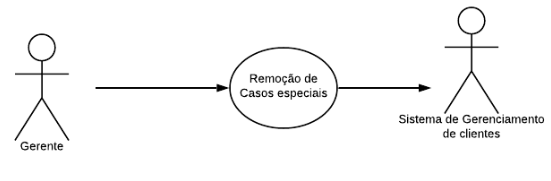
\includegraphics[width=1\textwidth]{pictures/removeespeciais.PNG} 
            \caption {Remoção de Casos Especiais} 
        \end{figure}
        
        \subsubsection{Cadastro de Funcionários}
        Uma hierarquia deverá ser obedecida para o gerenciamento de funcionários e clientes.
        \begin{figure}[H]
            \label{fig: cadastro} 
            \centering
            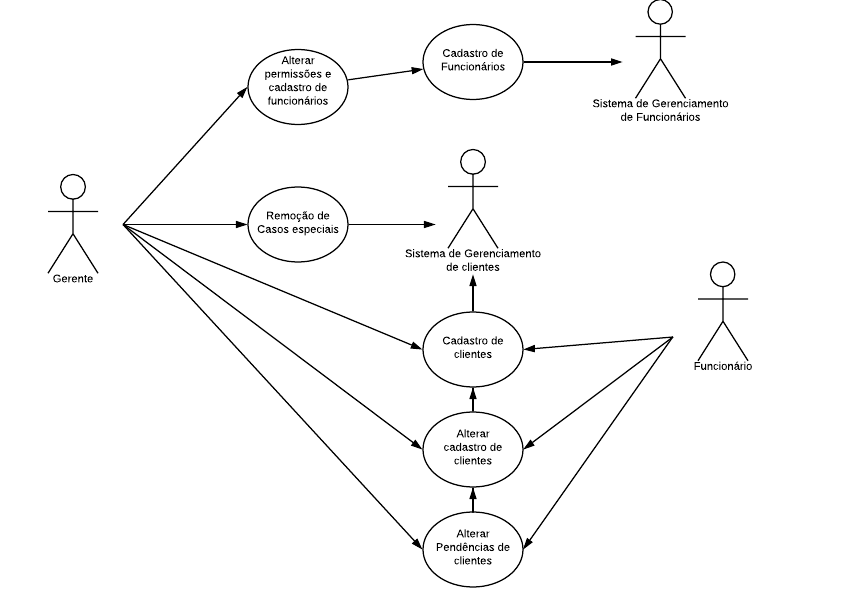
\includegraphics[width=1.0\textwidth]{pictures/cadastro.PNG} 
            \caption {Cadastro de Clientes e Funcionários} 
        \end{figure}        
        
        \subsubsection{Componentes do Sistema}
         O sistema será composto por outros sistemas individuais que trabalham em conjunto para o funcionamento do sistema como um todo.
        \begin{figure}[H]
            \label{fig: Diagrama de contexto} 
            \centering
            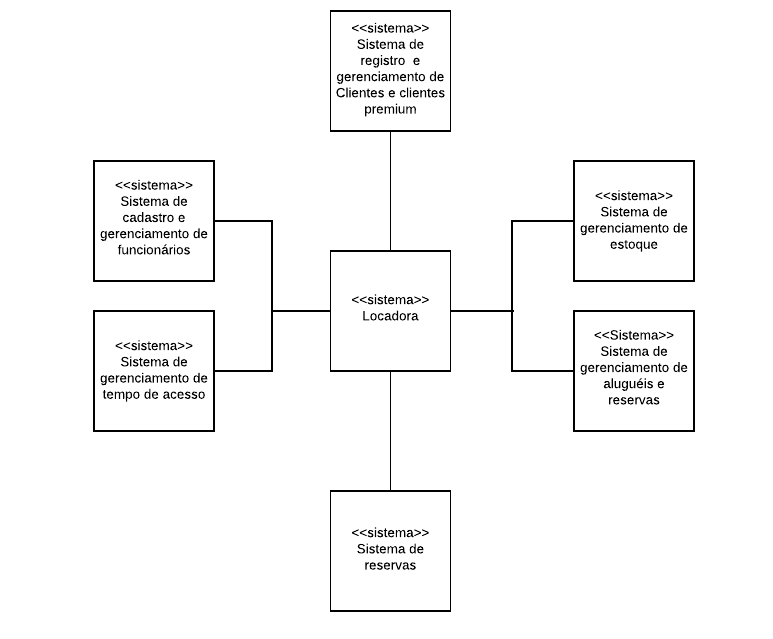
\includegraphics[width=1.0\textwidth]{pictures/contexto.PNG} 
            \caption {Componentes do sistema} 
        \end{figure}

         \subsubsection{Interface para Funcionários}
            A interface para funcionários deverá permitir o gerenciamento de clientes, tempos de jogo, registro de pagamentos, gerenciamento de estoque, entre outras atividades realizadas presencialmente na locadora e em caso de problemas com o sistema web ou mobile, deverá solucionar os mesmos auxiliando os clientes através de seu sistema.
            \begin{figure}[H]
                \label{fig: Diagrama de Casos de Uso}
                \centering
                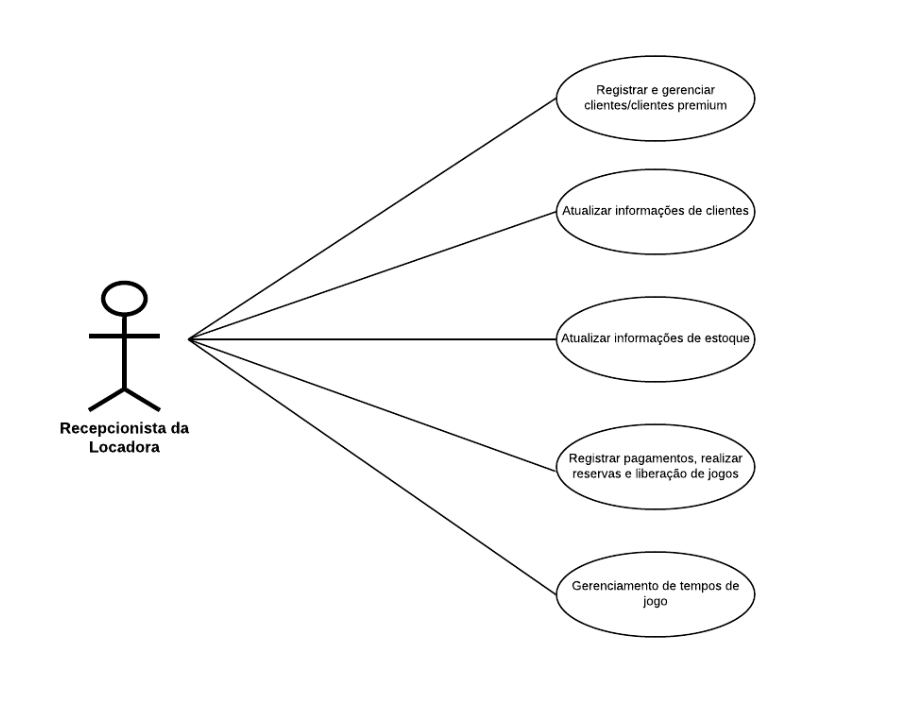
\includegraphics[width=.8\textwidth]{pictures/cduso.PNG} 
                \caption{Interface para funcionários}
            \end{figure}
            
             \subsubsection{Processo de Aluguel}
                O sistema deverá verificar disponibilidade de produtos e situação de clientes assim que for selecionado o produto para o aluguel, em caso de pendência ou casos especiais o mesmo deverá ser informado do motivo pelo qual o aluguel não foi permitido e quais os procedimentos necessários para resolver esse problema.
            \begin{figure}[H]
                \label{fig: Diagrama de processos} 
                \centering
                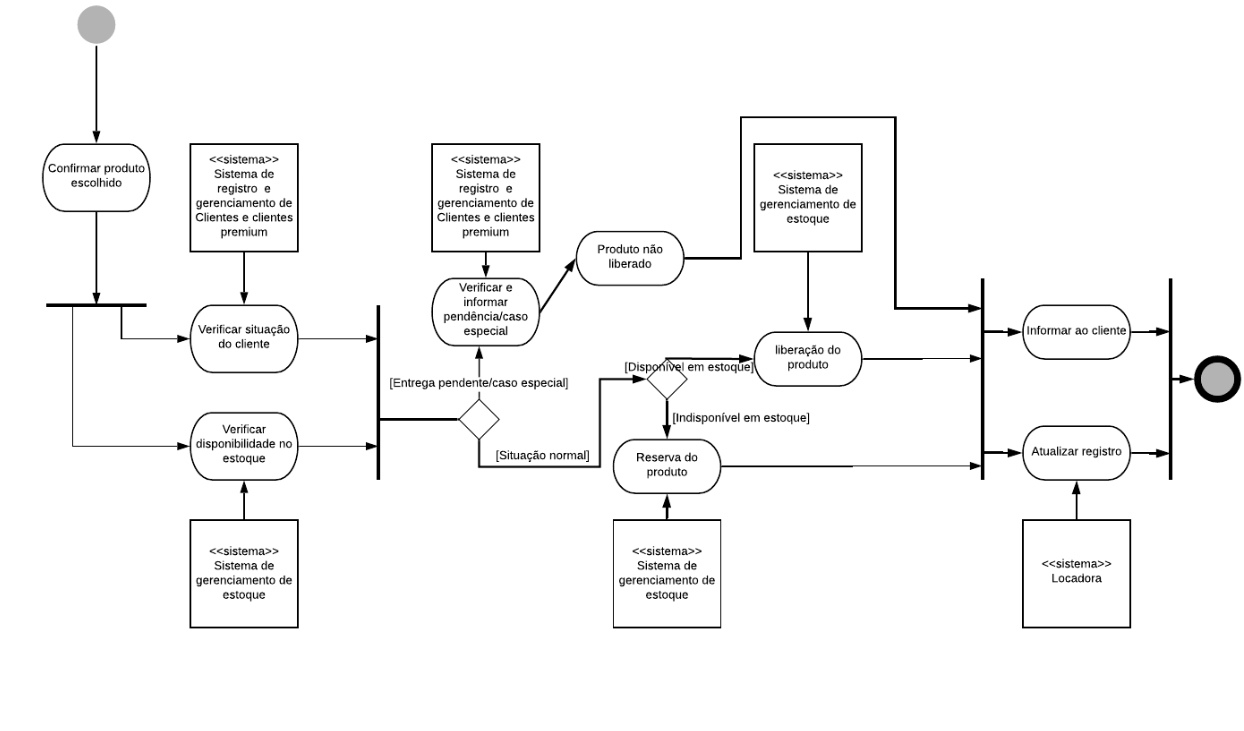
\includegraphics[width=.8\textwidth]{pictures/aluguel.PNG} 
                \caption{Processo de aluguel de um produto}
            \end{figure}
            
         \subsubsection{Remoção de Pendências}
            O funcionário poderá retirar restrições simples como pendência de entrega ou de pagamento de um cliente, no entanto em um caso especial, deve ser passado ao gerente para que o mesmo possa avaliar a situação e assim a melhor solução será escolhida com um acordo entre gerente e cliente.
            \begin{figure}[h]
                \label{fig: Diagrama de sequência} 
                \centering
                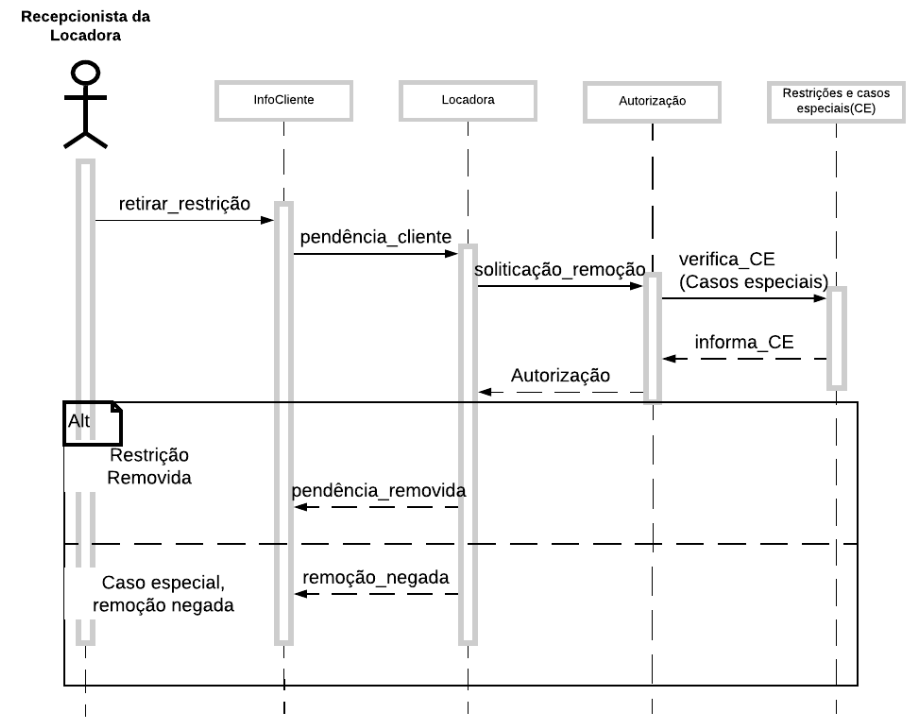
\includegraphics[width=1\textwidth]{pictures/especiais.PNG} 
                \caption{Processo de remoção de pendências}
            \end{figure}
    
    \subsection{Características do Usuário}
    %Descrever as características gerais dos usuários do produto.
    O sistema deverá ser usado por diversos tipos de clientes, como crianças sem conhecimento nenhum deixadas por seus pais para usar máquinas disponíveis na locadora, adolescentes com grande conhecimento em informática que vão usar máquinas na locadora ou alugar algum produto para usar em casa, adultos com conhecimento em informática que irão usar máquinas na locadora ou alugar algum produto ou mesmo adultos sem nenhum conhecimento que irão alugar produtos para seus filhos.\newline
    Para funcionários será exigido um nível mínimo de experiência e treinamento, o sistema será de fácil entendimento, porém deverá ter algumas ações mais complexas como retirar uma restrição, pendência ou cadastramento de um caso especial, apesar de sua simplicidade exigirá um pouco mais de conhecimento do usuário.
    
    
    \subsection{Restrições}
    %Descrever quais itens podem limitar as possibilidades do desenvolvedor.
    %Políticas organizacionais, criticalidade da aplicação,considerações sobre segurança, ...
    \subsection{Suposições e Dependências}
    %Listar os fatores que possam afetar os requisitos estabelecidos. Máquina específica, sistema operacional, ... 
    O sistema deverá ser desenvolvido para o funcionamento dividido em alguns sistemas:
    \begin{itemize}
        \item Windows 7 e 10: utilizado nas máquinas presentes no local para o uso de clientes, apenas necessário o sistema para gerenciamento de tempos.
        \item Android e IOS: utilizado por clientes para aluguéis, reservas e cadastros; não existindo necessidade de comunicação com o sistema de gerenciamento de tempos.
        \item Web: utilizado por clientes para aluguéis, reservas e cadastros; não existindo necessidade de comunicação com o sistema de gerenciamento de tempos.
        \item Linux: Utilizado pelo gerente e demais funcionários da locadora, necessário se comunicar com todos os outros sistemas, sendo assim o sistema principal.
    \end{itemize}
    
  \section{Requisitos Específicos}    
    %Contém todos os requisitos de software em um nível de detalhe.
        %Projetista seja capaz de projetar o sistema para satisfazer os requisitos.
    %Parte mais importante do documento.
    %Todos os requisitos devem ser identificados unicamente.
        %Atenção especial na organização dos requisitos para facilitar a leitura.
        
    \subsection{Interfaces Externas}        
    %Descrever detalhadamente todas as entradas e saídas do sistema.
    %Complementar as descrições das interfaces apresentadas na seção 2 do documento.
        %Interfaces com o usuário
        %Interfaces com hardware
        %Interfaces com software
        %Interfaces de comunicação
        
         % inicio das definições do documento
  \subsection{Definições}
    \FloatBarrier
    \begin{table}[H]
      \begin{center}
        \begin{tabular}[pos]{|m{5cm} | m{9cm}|} 
          \hline
          \cellcolor[gray]{0.9}\textbf{Termo} & \cellcolor[gray]{0.9}\textbf{Descrição} \\ \hline
          Requisitos Funcionais & Requisitos de hardware que compõem os módulos, descrevendo as ações que o mesmo deve estar apto a executar. Estas informações são capturadas a partir do desenvolvimento dos casos de uso, que documentam as entradas, os processos e as saídas geradas.  \\ \hline
          Requisitos Não Funcionais & Requisitos de hardware que compõem os módulos, representando as características que o mesmo deve ter, ou restrições que o mesmo deve operar. Estas características referem-se técnicas, algoritmos, tecnologias e especificidades do Sistema como um todo.  \\ \hline
        \end{tabular}
      \end{center}
    \end{table}  
  % fim

        
  % inicio da descriao de prioridades de requisitos
  \subsection{Prioridades dos Requisitos}
    \FloatBarrier
    \begin{table}[H]
      \begin{center}
        \begin{tabular}[pos]{|m{2cm} | m{12cm}|} 
          \hline
          \cellcolor[gray]{0.9}\textbf{Prioridade} & \cellcolor[gray]{0.9}\textbf{Característica} \\ \hline
          Importante      & Requisito sem o qual o sistema funciona, porém não como deveria.  \\ \hline
          Essencial       & Requisito que deve ser implementado para que o sistema funcione.  \\ \hline
          Desejável       & Requisito que não compromete o funcionamento do sistema.  \\ \hline
        \end{tabular}
      \end{center}
    \end{table}  
  % fim
  
  % inicio dos requisitos funcionais
  \subsection{Requisitos Funcionais}
    \begin{functional}
     % \requirement{name}{description}{priority}
     \requirement
      {Armazenamento de estoque}
      {Armazena o estoque com os detalhes de cada produto e é atualizado a cada entrada ou saída de produtos.}
      {Essencial}

     \requirement
      {Cadastro e gerenciamento de clientes}
      {Cadastra o cliente e suas informações básicas (RG, CPF, nome completo, endereço, etc.), armazena os aluguéis (interagindo diretamente com o estoque) e casos especiais (atrasos, avarias no produto, não devolução, etc.)}
      {Essencial}

     \requirement
      {Cadastro e gerenciamento de funcionários}
      {Armazena as informações de cada funcionário, horário de chegada e saída, suas permissões e restrições, atividades realizadas no dia, etc.}
      {Essencial}
    \end{functional}
  
    \begin{functional}
      \requirement
      {Gerenciamento de tempos}
      {Gerencia o tempo de uso das máquinas e consoles no local armazenando o tempo disponível para o uso, com um aviso com alguns minutos restantes e finalizando automaticamente a sessão após o término do mesmo.}
      {Importante}
      
    \requirement
      {Sistema de notificações}
      {O cliente poderá colocar jogos a serem lançados em uma lista de favoritos, realizar reservas e será notificado quando o produto desejado ficar disponível. O cliente também será notificado com antecedência para a devolução do produto.}
      {Importante}

     \requirement
      {Reserva de produto}
      {Em caso de lançamento de jogo ou falta do produto em estoque, uma reserva do produto deve ser feita e assim que disponível em estoque deverá ser notificado ao cliente.}
      {Essencial}
      
   
      \requirement
      {Plano de usuário premium}
      {Sistema de fidelidade que pode gerar prioridade em filas para o aluguel, descontos, frete grátis caso opte pela entrega, etc.}
      {Desejável}

      \requirement
      {Categorização de jogos}
      {Os jogos deverão ser divididos em categorias que influenciarão diretamente no valor de aluguel e quantidade em estoque, dividindo os jogos com base na demanda.}
      {Desejável}
      
      \requirement
      {Catálogo}
      {Um catálogo contendo todos os jogos e sua disponibilidade deverá ser gerado e o mesmo deverá ser atualizado em tempo real a cada aluguel ou devolução, informando a quantidade de produtos disponível e sua fila de espera}
      {Importante}
      
      \requirement
      {Situação de produtos}
      {Um produto novo ou devolução deverá ter em seu cadastro um campo para especificar sua situação que deverá ser avaliada através de testes.}
      {Importante}

    \end{functional} 
 
\subsection{Requisitos não Funcionais}
% Esta seção apresenta a lista de Requisitos não Funcionais do projeto.

  \begin{nonfunctional}
    \requirement
    {Cadastros restritos}
    {Não permitir aluguéis para clientes com devoluções pendentes ou processos de casos especiais.}
    {Importante}
    
    \requirement
    {Gerenciamento de Casos especiais}
    {Apenas o gerente terá permissão para retirar ou alterar casos especiais, assim caso haja a necessidade de alteração ou remoção do mesmo, deverá ser passado ao gerente.}
    {Importante}
    
    \requirement
    {Hierarquia de gerenciamento}
    {Apenas o gerente terá permissão para alterar cadastros de funcionários, impedindo assim a alteração cadastral pelos próprios funcionários, com exceção de casos especiais, os funcionários terão autonomia para o gerenciamento de clientes e os clientes poderão alterar apenas os próprios dados cadastrais como: nome, documentos, endereço, etc.}
    {Importante}
    
    \requirement
    {Cadastro responsável}
    {Não permitir o cadastro de menores não acompanhados pelos pais ou responsáveis no estabelecimento. Caso acompanhados, deve-se cadastrar com os documentos do menor e de seu responsável.
    No caso de cadastro pelo aplicativo, permitir apenas o cadastro de maiores.}
    {Importante}

    \requirement
    {Aluguéis para terceiros}
    {Não permitir aluguel para terceiros não autorizados previamente e cadastrados na ficha do cliente requerido.}
    {Importante}

    \requirement
    {Restrição de horário}
    {Não permitir o login de menores de 16 anos no local após as 22h.}
    {Desejável}
    
    \requirement
    {Período letivo}
    {Durante o período letivo, exceto por férias, finais de semana e feriados, não permite o login de estudantes em seu horário de aulas.}
    {Desejável}
    
    \requirement
    {Aluguel Responsável[PRESENCIAL]}
    {Não permitir o aluguel de jogos adultos ou violentos para menores sem a presença dos responsáveis.}
    {Desejável}
    
    \requirement
    {Teste de jogos}
    {Novos produtos e produtos devolvidos só poderão ser novamente ser inseridos no estoque após serem testados e avaliados.}
    {Importante}
    
  \end{nonfunctional}
    \subsection{Requisitos de Desempenho}
    %Descrever as características de desempenho que o sistema deve atender.
    %Número de usuários simultâneos.
    %Utilização de recursos (memória, disco, ...).
    %Tempo de resposta de uma transação.
    %Número de transações e tarefas a serem processadas dentro de certo período de tempo, em condições normais e de sobrecarga. 
                    
                    %95% das transações devem ser processadas em menos de 1 segundo.
                                %X
                %Um usuário não deve ter que esperar para que as transações sejam completadas.
    O sistema deverá processar simultaneamente vários alugueis, acessos às maquinas presentes no local simultaneamente, atualizando o estoque, situações de clientes, casos especiais, e  evitando situações como:
      \begin{itemize}
        \item \textbf{Alugueis de produtos indisponíveis} - O último produto disponível foi alugado e não houve atualização do estoque
        \item \textbf{tentativa de aluguel falha por pendência inexistente} -  Em casos de devolução realizada e ainda não computada.
        \item \textbf{Aluguel para clientes com pendências e casos especiais} - Em casos de atraso ou CE não atualizado no banco de dados.
        \item \textbf{Aviso de disponibilidade} - Em casos de reservas, o primeiro cliente da fila de espera não foi notificado imediatamente.
        \item \textbf{Término de tempo} - As máquinas disponíveis no local deverão ser restringidas imediatamente ao término do tempo do usuário e notificar o funcionário neste momento para evitar que usuários utilizem as mesmas além do tempo pago.
        \item \textbf{Atualização de estoque} - Em casos onde novos produtos são adicionados ao estoque, disponibilizar imediatamente no catálogo diminuindo filas de espera.
        \item \textbf{Processamento de transações} - Transações devem ser processadas em menos de 5 segundos, um cliente não deve ter de esperar para que as transações sejam completas.
        \item \textbf{Acesso de ex-funcionários} - Desativando o cadastro de antigos funcionários imediatamente para evitar acesso ao banco de dados da locadora.
  \end{itemize}
    %\subsection{Requisitos Lógicos de Banco de Dados}   
    %Descrever os requisitos para qualquer informação a ser colocada na base de dados.
        %Tipo da informação usada por várias funções.
        %Frequência de uso.
        %Capacidade de acesso.
        %Entidades de dados e seus relacionamentos.
        %Restrições de integridade.
        
    %\subsection{Restrições de Projeto}    
    %Descrever restrições de projeto impostas por outros padrões, limitações de hardware, etc.
    %\subsection{Suposições e Dependências}  
    %Listar todos os fatores que afetam os requisitos da especificação. Esses fatores não são restrições ao projeto do sistema, mas sim mudanças que podem afetar os requisitos. Por exemplo, um suposição pode ser que a aplicação será instalada em um sistema operacional específico. Se, este sistema operacional não for disponível, isso poderia afetar os requisitos.
    %\section{Anexo}  
    %Citar todos os recursos e técnicas utilizados para a extração de requisitos, assim como as questões feitas, o nome das pessoas, empresas, telefones e datas de contato.
    \subsection{Casos de risco}
    Durante o processo de desenvolvimento do sistema, riscos serão considerados para evitar problemas futuros e imprevistos.
        \FloatBarrier
    \begin{table}[H]
      \begin{center}
        \begin{tabular}[pos]{|m{2.55cm}| m{1.2cm}| m{3.6cm}| m{6cm}|} 
          \hline
          \cellcolor[gray]{0.9}\textbf{Situações} & \cellcolor[gray]{0.9}\textbf{Risco} &
          \cellcolor[gray]{0.9}\textbf{Problema} &
          \cellcolor[gray]{0.9}\textbf{Solução} \\ \hline
          Equipe Doente & Alto & Membro da equipe e precisa se afastar de suas atividades por um período de tempo. & Os componentes deverão ser desenvolvidos de forma conjunta, em que membros da equipe estejam cientes das tarefas de seus colegas para, em casos onde seja necessário um membro faltar, seu colega de equipe consiga prosseguir com seu projeto de forma individual.  \\ \hline
           Atraso de projeto & Médio & Devido a algum fator, como erros ou imprevistos, o tempo de entrega será maior do que o esperado. & O cálculo de tempo deverá ser feito de forma que não seja longo demais mas não seja o tempo exato que o projeto leva para ser concluído, assim reservando tempo para correção de possíveis problemas. Além do backup do projeto que deverá ser realizado regularmente. \\ \hline
           Diminuição de investimento & Baixo & Devido a algum problema financeiro o investimento do projeto deverá ser reduzido. & O projeto deverá trabalhar com membros temporários na equipe que em casos extremos poderão ser desligados, se necessário. \\ \hline
            Conflitos de sistemas & Alto & Algum dos sistemas que compõem o sistema principal entra em conflito com alguma restrição ou permissão. & Os sistemas serão desenvolvidos de forma separada e com backups realizados regularmente, de forma que um conflito possa ser realizado facilmente identificado e corrido. \\ \hline
        \end{tabular}
      \end{center}
    \end{table}  
  % fim
  
% Optional bibliography section
% To use bibliograpy, first provide the ipprocess.bib file on the root folder.
% \bibliographystyle{ieeetr}
% \bibliography{ipprocess}

\end{document}